\section{Character and number encodings}
\label{sec:characters}

\begin{quotation}%
\verb|Breakdowns : portrait of the artist as a young %@[squiggle][star]!| \\
\quotationsource
Unknown library cataloger, titling a book by \Person[Art]{Spiegelman}
\end{quotation}

% Breakdowns : Portrait des Künstlers als junger %@[Schnörkel][Stern]!
% Kommentar: In der Vorlage "Schnörkel" und "Stern" als Symbol wiedergegeben

\noindent All data must be written down in some form. At least a standardized
set of base symbols (\Term{character}s) is needed together with a set of
conventions how to meaningfully combine these symbols. We call this two sets a
\Term{writing system} or \term{notation}.  The connection of data and writing
systems is not an invention of the digital age: Cuneiform script on clay
tablets, the earliest known records of a writing system from the 4th millennium
BC, was first used exclusively for accounting and record keeping, thus for
capturing data.  The simplest writing system can only write down sequences of
binary data. It consists of two distinct symbols (usually called zero and one),
and the convention of concatenating these symbols to sequences. More complex
writing systems involve more characters. A \Term{character encoding} maps
characters and their combination rules to a writing system on symbols that can
easier be stored and communicated. Examples of character encodings include
Morse code, Braille, the \tacro{American Standard Code for Information
Interchange}{ASCII}, and \term{Unicode}. Digital character encodings map
characters to a sequence of bits. Before Unicode became the dominant character
encoding standard (starting in the early 1990s), there were many alternative
encodings for different sets of characters. Table~\ref{tab:aringencodings}
lists some pre-Unicode encodings and their mappings of the capital letter
\r{A}:

\begin{table}[h]
\centering
\begin{tabular}{l|r|r}
 \textbf{encoding} & \textbf{hexadecimal} & \textbf{binary} \\
\hline
 US-ASCII           & --- & --- \\
\hline
 ISO~646 DK/NO/SE   & \verb|5D| & \verb| 1011101| \\
\hline
 EBCDIC CP37 etc.   & \verb|67| & \verb|01100111| \\
\hline
 Mac~OS~Roman       & \verb|81| & \verb|10000001| \\
\hline
 Allegro-DOS/IBM437 & \verb|8F| & \verb|10001111| \\
\hline
 NeXTSTEP           & \verb|86| & \verb|10000110| \\
\hline
 ISO 8859-1         & \verb|C5| & \verb|11000101| \\
\hline
 ANSEL (MARC-8) combining \r{} + A & \verb|EA 41| 
  & \verb|11101010 01000001| \\
\end{tabular}
\caption{Various character encodings of the capital letter \r{A}}
\label{tab:aringencodings}
\end{table}

\subsection{Unicode}
\label{sec:Unicode}

Unicode aims at unifying all binary character encodings by covering all
characters for all writing systems of the world, modern and ancient
\cite{Unicode6}. The standard includes graphemes and grapheme-like units like
punctuations, technical symbols, and many other characters used in writing
text. The Unicode standard defines a \Term{grapheme} as ``a minimally
distinctive unit of writing in the context of a particular writing system.'' or
``what a user thinks of as a character''.  For instance the lines in
example~\ref{ex:loremipsum} consist of equal sequences of graphemes in Unicode
because typographic differences do not matter.

\begin{example}
\centering
\includegraphics[width=3cm]{img/loremipsum.jpg}
\caption{Equal sequences of graphemes (if encoded in Unicode) }
\label{ex:loremipsum}
\end{example}

In contrast to earlier systems, Unicode also covers multiple combination
rules, such as combining diacritics, bidirectional text, line and paragraph
separators etc. Unicode even included language tags --- special characters to
identify text as belonging to a particular language --- but this practice has
been marked as deprecated in favor of \term{markup language}s. The following
analysis of character encodings focuses on Unicode. It is referenced in many
other standards, and most characters of any other other relevant digital
character encoding are also located at some place in Unicode. Unicode is
explicitly designed as open, evolving standard.  New versions do not remove or
change characters, but only add new characters and possibly change character
properties after careful deliberation. That explicitly makes any possible
abstract character a potential candidate for inclusion in the Unicode standard.
To do so, one can define character mappings in private use areas, but there is
no standard way to tell external applications about appearance and other
properties of the corresponding graphemes. For this reason the use of Unicode
is limited to symbols that are officially accepted as graphems in the standard
--- for instance \term{written sign language} \cite{Sutton2002} and other
two-dimensional notations are not included.  The set of characters encoded in
Unicode is called the \Tacro{Universal character set}{UCS} and the set of
symbols, which is a subset of the integer values, is called the \Term{Unicode
code point}s (\format{codepoint}) in table~\ref{tab:unicode}).  All Unicode
code points are located in the range \Ox{00} to \Ox{10FFFF} which theoretically
makes 1,114,112 possible values, expressible in 21 bit. A Unicode code points
is referred to in documentation by writing `\U{}' before its value in
hexadecimal notation. By now, most code points are not assigned\footnote{As of
Unicode~6.0.0 there are 109,449 assigned graphical characters, 207 special
purpose characters for control and formatting, and 142,999 reserved for private
use.} and 2,114 values are explicitly excluded: the \term{surrogates} \U{D800}
to \U{DFFF} and 66 special \format{noncharacter} codes  are permanently
reserved for internal use. They are forbidden for use as character code point
in \acro{UCS} and in open interchange of Unicode text data
(table~\ref{tab:unicode}).

% surrogates: %\cite[section 16.6]{Unicode6} 
% noncharacters: %\cite[section 16.7]{Unicode6}

\begin{table}[ht]
\begin{lstlisting}[language=BNF]
 codepoint    = [#x00-#x10FFFF]
 surrogate    = [#xD800-#xDFFF]
 ustring      = ( codepoint - surrogate )*
 noncharacter = [#xFDD0-#xFDEF] | #xFFFE |#xFFFF |#x1FFFE|#x1FFFF|
  #x2FFFE|#x2FFFF|#x3FFFE|#x3FFFF|#x4FFFE|#x4FFFF|#x5FFFE|#x5FFFF| 
  #x6FFFE|#x6FFFF|#x7FFFE|#x7FFFF|#x8FFFE|#x8FFFF|#x9FFFE|#x9FFFF| 
  #xAFFFE|#xAFFFF|#xBFFFE|#xBFFFF|#xCFFFE|#xCFFFF|#xDFFFE|#xDFFFF|
  #xEFFFE|#xEFFFF|#xFFFFE|#xFFFFF|#x10FFFE|#x10FFFF
\end{lstlisting}
\caption{Symbol ranges in Unicode}
\label{tab:unicode}
\end{table}

Unicode characters are not directly mapped to binary sequences. Instead the
standard defines a number of encodings such as UTF-8, UTF-16 etc. to map
\format{ustring} to sequences of Bytes. The mapping is neither injective, nor
surjective or functional. Table~\ref{tab:utfaringencodings} lists several
schemes that all encode the capital letter \r{A}. The abbreviations `LE' and
`BE' indicate the byte order little-endian (default) and big-endian.  Different
combinations of UTF-8, UTF-16, UTF-32, or UTF-EBCDIC\footnote{UTF-EBCDIC was
defined to better support mainframe EBCDIC computers, which nowadays may only
be found in archaic systems, like nuclear power plants.} with BE or LE define
alternative transformation formats.  They can easily be mapped to each other as
isomomorphic encodings of \acro{UCS}. A full breakdown of the encoding of the
composed character is provided with example~\ref{ex:Aring} in
section~\ref{sec:levels}.

% on UTF-8
% http://www.cl.cam.ac.uk/~mgk25/ucs/utf-8-history.txt
% created by Ken Thompson

\begin{table}[h]
\centering
\begin{tabular}{l|r|r}
 \textbf{Unicode encoding scheme} & \textbf{hexadecimal} & \textbf{binary} \\
\hline
 UTF-16, LE: \r{A}ngstr\"{o}m sign & \verb|21 2B| 
& \verb|00100001 00101011| \\
\hline
 UTF-16, BE: \r{A}ngstr\"{o}m sign & \verb|2B 21|
& \verb|00101011 00100001| \\
\hline
 UTF-16, LE: \r{A} & \verb|00 C5|
& \verb|00000000 11000101| \\
\hline
 UTF-8, LE: \r{A} & \verb|C3 85|
& \verb|11000011 10000101| \\
\hline
 UTF-16, LE: A + combining \r{} & \verb|00 41 03 0A| 
& \verb|00000000 01000001| \\
& & \verb|00000011 00001010| \\
\hline
 UTF-8, LE: A + combining \r{} & \verb|41 CC 8A| 
& \verb|01000001 11001100| \\ & &  \verb|10001010| \\
\end{tabular}
\caption{Various Unicode encoding schemes encoding the capital letter \r{A}}
\label{tab:utfaringencodings}
\end{table}

As described by \textcite{Davis2010}, Unicode does not directly encode
characters in UCS but it encodes graphemes, which may be combined to grapheme
clusters as user-perceived characters. In general each graphem should be
assigned to exactly one Unicode code point. For historical reasons there are
some exceptions, like \U{00C5} (latin capital letter a with ring above) and
\U{212B} (angstrom sign). One may argue that both are different characters, if
used in different context, but as they both map to the same visible grapheme,
the difference is difficult to sustain. Some same grapheme clusters can be
created by multiple sequences of codepoints. For this reason the Unicode
standard defines two kinds of equivalence between code point sequences:
\Term[canonical equivalence (Unicode)]{canonical equivalence} and
\Term[compatible equivalence (Unicode)]{compatible equivalence}. Canonical
equivalence is based on \term[character (de)composition]{character
composition}, that is the process of combining multiple characters to one ---
the reverse process is called decomposition. A combined character sequence and
its canonical equivalent precomposed character should always have the same
visual appearance and behaviour. Compatible equivalence is based on minor
visual differences, that may be significant in some contexts only. Examples of
compatible equivalences are font variants, ligatures, and digraphs.
Composition and decomposition are mappings that ground on character properties
of the Unicode character database. Given these mappings, there are four
official \term{normalization} forms \cite{David2009}: %
\url{http://unicode.org/reports/tr15/} \tacro{Normalization Form D}{NFD}
transforms a string by mapping each character to its canonical decomposition.
\tacro{Normalization Form C}{NFC} first decomposes all characters with
\acro{NFD} and then transforms the resulting string by canonical composition.
For instance a string that contains the letter \r{A} in any of the forms
\U{212B}, \U{C5}, and \U{41} followed by \U{038A} will only contain it as
\U{C5} after \acro{NFC}.  \tacro{Normalization Form KD}{NFKD} transforms a
string by compatible decomposition and \tacro{Normalization Form KC}{NFKC} adds
canonical (sic!) composition after compatible decomposition. \acro{NFKD}
subsumes \acro{NFD} and \acro{NFKC} subsumes \acro{NFC}.  Normalization also
provides a unique order for combining marks, so it can be used to determine
string equivalence. Once normalized, a string should not change when normalized
again with the same operation.\footnote{This implies that equivalence mappings
of a given character cannot be changed in future versions of Unicode. The
stability guarantee on normalization only applies to assigned characters in
\acro{UCS}.} None of the normalization forms is bijective (fully reversible)
because each maps the set \format{ustring} to a smaller subset.

On a closer look, Unicode contains many inconsistencies and exceptions in
respect to character properties and normalization. For example Chinese
characters are composed of strokes, but there is no decomposition mapping
to the set of strokes which form a given chinese character. Some icons,
ligatures and digraphs are included in \acro{UCS} but others are rejected,
even if used as distinct graphemes.\footnote{For instance one method of writing
the M\=aori language in the early 20th century contained a special `wh' ligature
as distinct character. Although there are printed books that use this letter,
it was rejected for inclusion in Unicode. See 
\url{http://unicode.org/faq/ligature_digraph.html} for the objections of 
Unicode Consortium in ligatures and digraphs. Icons and pictograms are
reluctantly included as well, but Unicode version 6.0 introduced
several hundred Emoji icons for animals, clothes, vehicles, food and other
random artifacts. The history including the capital sharp s, rejected in
2004 but included as \U{1E9E} in Unicode version 5.1.0 after a second
proposal, reveals some interesting insight into the process of standardization.}
Said that, one must keep in mind that the aim of Unicode is not to create an
objective model of all human writing systems but to ensure compatibility in
exchange of character strings. In addition to composition properties, the
character database contains a large number of attributes to describe
relevant characteristics and relations like character type, case, order
etc. \cite{Whistler2008}. However this metadata is relatively static and
excludes many aspects like historical relations and visual similarities.
Based on character properties, applications can define custom
normalization forms, for instance \acro{NFKD} followed by
lowercase case-folding and removal of all diacritics.

While Unicode is the dominant standard for character encoding on the level of
byte sequences, there are other methods that express characters as sequences
of other characters or symbols (see table~\ref{tab:otheraringencodings}).
Some encodings are not reversible because they map multiple characters to the
same symbols. Problems frequently arise, if data include symbols without known
character encoding or if different creators and users of data do not agree on
a common character encoding and interpretation.

\begin{table}[h]
\centering
\begin{tabular}{l|l}
 \textbf{encoding} & \textbf{symbols} \\
\hline
 named HTML entity & \verb|&Aring;| \\
\hline
 XML character entity & \verb|&#xc5;|, \verb|&#xC5;|, \verb|&#197;|,
\verb|A&#x030A;| \ldots \\
\hline
 Swedish 6 dot Braille & 
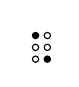
\begin{tikzpicture}[baseline]
   \path[use as bounding box] (-1mm,0) (2mm,0) (2mm,4mm);
   \draw ( 0, 0) circle (.4mm);
   \draw ( 0,.15) circle (.4mm);
   \draw[fill] ( 0,.30) circle (.4mm);
   \draw[fill] (.15, 0) circle (.4mm);
   \draw (.15,.15) circle (.4mm);
   \draw (.15,.30) circle (.4mm);
 \end{tikzpicture} 
~pattern P16 (Unicode \U{2821})
\\ \hline
Eurobraille 8 dot&
 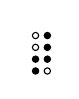
\begin{tikzpicture}[baseline]
   \path[use as bounding box] (-1mm,0) (2mm,0) (2mm,5.5mm);
   \draw[fill] ( 0, 0) circle (.4mm);
   \draw[fill] ( 0,.15) circle (.4mm);
   \draw ( 0,.30) circle (.4mm);
   \draw ( 0,.45) circle (.4mm);
   \draw (.15, 0) circle (.4mm);
   \draw[fill] (.15,.15) circle (.4mm);
   \draw[fill] (.15,.30) circle (.4mm);
   \draw[fill] (.15,.45) circle (.4mm);
 \end{tikzpicture} 
~pattern P34567 (Unicode \U{287C})
\\ \hline
Transcription & Aa
\\ \hline
Morse code (\r{a} = \`{a}, no case) & $\cdot$ - - $\cdot$ - \\
\end{tabular}
\caption{Additional character encodings of \r{A}}
\label{tab:otheraringencodings}
\end{table}

% Some sources:
% NeXT
%  http://unicode.org/Public/MAPPINGS/VENDORS/NEXT/NEXTSTEP.TXT
% IBM EBCDIC
%  http://www.unicode.org/Public/MAPPINGS/VENDORS/MICSFT/EBCDIC/CP037.TXT
%
% ANSEL: combining ring above (EA) + A (41)
% US-ASCII, ISO~646 (7-bit with national variants)
% ISO~8859 (8-bit)

% (see \cite{Whistler2008} \url{http://unicode.org/reports/tr23/} for 
% a metamodel of Unicode properties).

\subsection{Number encodings}
\label{sec:numberencodings}

A typical misconception about computers is that they deal with numbers, but
they only deal with bits.  Sequences of bits are used to encode numbers, just
like character encodings encode characters. In contrast to arbitrary
characters, the \term{value space} of numbers includes a mathematical model,
that defines algebraic operations for calculation (see
section~\ref{sec:datatypes}).  Digital number encodings should support these
operations on representations of numbers, but they are typically defined on a
limited computational model. First of all, most number systems are infinite
while most number encodings limit each number to a fixed number of bits. The
most prominent types of number encodings are integers, floating point numbers,
and possibly boolean data types which map one bit to one boolean value (true or
false).

\Term{Integer} data types represent (a subset of) the integer numbers
$\mathbb{Z}=\set{\ldots-2,-1,0,1\ldots}$. One can encode $\mathbb{Z}$ (up to
limits of memory) by using a variable size encoding like used for instance in
the Protocol Buffers data binding language \cite{Varda2008}.  In practice most
integer data types have some fixed size of $n$ bits that store an integer value
in binary numeral system.  The range that can be encoded with $n$ bit is
$-2^{n-1}$ to $2^{n-1}-1$ for signed integers ($\format{Int}_{n}$) and $0$ to
$2^n-1$ for unsigned integers ($\format{UInt}_{n}$).

There are several encodings for subsets of the real numbers $\mathbb{R}$ with
\Term{floating point} data types as most common method.  The basic idea of
floating point numbers is to represent a real number $r$ as the result $r = m
\cdot b^x$ with two integer components, exponent $x \in \mathbb{Z}$, and
mantissa $m \in \mathbb{Z}$, and a base $b$. For example with base $b=10$ the
number $374.2$ could be represented as $3742 \cdot 10^{-1}$. The mapping allows
for multiple encodings of the same number, for instance $374.2$ is also $37420
\cdot 10^{-2}$. For this reason floating point numbers are typically stored in
normalized form where the mantissa must be in a specific range. In digital encoding, 
the base of most floating point encodings is $b=2$. The exponent is typically 
stored as unsigned integer with a fixed bias value and one can save the first bit 
of the mantissa by assuming that it must always be $1$ for normalized numbers.
Calculation with floating point numbers is tricky because there are several ways
in which the result of a calculation may not be part of the selected subset of 
$\mathbb{R}$. This can also happen in integer encodings but floating point 
encodings often support special values for this cases, such as signed zeroes 
($-0$ and $+0$ are encoded as different values), infinities ($+\inf$ and $-\inf$ 
are allowed), and ``not a number'' values (NaN). IEEE~754 \cite{ieee2008}, the
most popular floating point encoding, distinguishes between two kinds of NaN, 
quiet NaN and signaling NaN. However, there is no portable way to assign the second
as data value because either it is converted to a quiet NaN or an exception is 
raised. Furthermore IEEE~754 and related standards still allow for some variations 
in implementations that can led to different results, depending on the computer
platform \cite{Monniaux2008}.\footnote{Under specific circumstances a floating
point variable may even change its encoding without an assignment to it.}
In summary one must take care which specific floating encoding one deals with or
better avoid floating point values in favor of other encodings like
decimal notation with arbitrary precision or symbolic notation.
